\documentclass[10pt, a4paper]{report}

\usepackage[utf8]{inputenc}
\usepackage{polski}
\usepackage{a4wide}
\usepackage{fancyhdr}
\usepackage{lastpage}
\usepackage{tabularx}
\usepackage{graphicx}
\usepackage{listings}
\usepackage{forest}
\usepackage{xcolor}


\graphicspath{ {./images} }

\definecolor{folderbg}{RGB}{124,166,198}
\definecolor{folderborder}{RGB}{110,144,169}
\definecolor{codegreen}{rgb}{0,0.6,0}
\definecolor{codegray}{rgb}{0.5,0.5,0.5}
\definecolor{codepurple}{rgb}{0.58,0,0.82}
\definecolor{backcolour}{rgb}{0.95,0.95,0.92}

\lstdefinestyle{listings}{
    backgroundcolor=\color{backcolour},   
    commentstyle=\color{codegreen},
    keywordstyle=\color{magenta},
    numberstyle=\tiny\color{codegray},
    stringstyle=\color{codepurple},
    basicstyle=\ttfamily\footnotesize,
    breakatwhitespace=false,         
    breaklines=true,                 
    captionpos=b,
    keepspaces=true,                 
    numbers=left,                    
    numbersep=6pt,                  
    showspaces=false,                
    showstringspaces=false,
    showtabs=false,                  
    tabsize=4
}

\def\Size{4pt}
\tikzset{
  folder/.pic={
    \filldraw[draw=folderborder,top color=folderbg!50,bottom color=folderbg]
      (-1.05*\Size,0.2\Size+5pt) rectangle ++(.75*\Size,-0.2\Size-5pt);  
    \filldraw[draw=folderborder,top color=folderbg!50,bottom color=folderbg]
      (-1.15*\Size,-\Size) rectangle (1.15*\Size,\Size);
  }
}

\begin{titlepage}
    \title{\huge{\textbf{Specyfikacja funkcjonalna} \\ programu \textit{"grapher"}}}
    \author{Szymon Półtorak i Sebastian Sikorski}
    \date{21.04.2022r}
\end{titlepage}

\renewcommand{\footrulewidth}{1pt}
\lstset{style=listings}

\begin{document}
    \maketitle
    \renewcommand*\thesection{\arabic{section}}

    \begin{abstract}
      Celem dokumentu jest zawarcie informacji dotyczących programu, omówienie struktury folderu, funkcjonalności programu oraz jego uruchomienie.
      Dzięki temu dokumentowi użytkownik może zapoznać się z tematem projektu oraz najistotniejszymi informacjami dotyczącymi projektu. Niniejszy dokument jest przede wszystkim instrukcją obsługi
      programu \texttt{grapher}. Pokazujemy obsługiwane błędy, wyjaśniamy ich kody oraz komunikaty.
    \end{abstract}

    \pagestyle{fancy}
    \fancyhf{}
    \lhead{Specyfikacja funkcjonalna programu \textit{grapher}(Java)}
    \rhead{Szymon Półtorak i Sebastian Sikorski}
    \cfoot{Strona \thepage \hspace{1pt} z \pageref{LastPage}}
    
    \fancypagestyle{plain}{
        \lhead{Specyfikacja funkcjonalna programu \textit{grapher}(Java)}
        \rhead{Szymon Półtorak i Sebastian Sikorski}
        \cfoot{Strona \thepage \hspace{1pt} z \pageref{LastPage}}
    }
    \tableofcontents
    \newpage

    \section{Podstawowe informacje}
    \subsection{Przeznaczenie programu}
    Program został napisany z myślą o osobach pracujących z grafami typu \textit{karta w kratkę}. Pozwala on generować graf w trzech trybach, które
    zostaną wyjaśnione w podrozdziale \textit{Cel projektu}.

    \subsection{Wymagania programu}
    Program \textit{grapher} jest programem pisanym z myślą o współpracy z systemami operacynymi \textit{MacOS} oraz \textit{Windows}.
    Prawidłowe działanie programu wymaga posiadania środowiska uruchomieniania Javy (\textit{Java Runtime Enviroment}) służącego do uruchamiania program o rozszerzeniu \textit{.jar} lub środowiska
    programistycznego wraz z odpowiednim \textit{Java Development Kit} oraz \textit{JavaFX}.

    \subsection{Cel Projektu}
    Celem projektu było stworzenie programu mającego za zadanie generowanie grafów, sprawdzanie ich spójności oraz wyszukiwanie w nich najkrótszej ścieżki między zadanymi przez użytkownika punktami. 
    Grafi są typu \textit{kartka w kratkę}.

    \begin{itemize}
        \item Wage Mode – program generuje graf o losowych wagach dróg między wierzchołkami w taki sposób, że jest on spójny,
        \item Edge Mode – program losuje istnienie krawędzi między wierzchołkami grafu oraz wagi do momentu powstania 
        grafu spójnego. Do sprawdzania wykorzystuje algorytm przeszukiwania wszerze (BFS),
        \item Random Mode – program losuje wagi dróg oraz krawędzie między wierzchołkami. W tym trybie graf może być niespójny,
        \item Read Mode -- program odczytuje odpowiednio sformatowany plik i szuka najkrótszej ścieżki
        między podanymi przez użytkownika punktami za pomocą algorytmu Dijkstry. Jeżeli użytkownik poda w pliku nieprawidłowe dane
        tzn. wprowadzi literę zamiast wierzchołka lub wagi albo nie poda wierzchołka, a poda wagę i na odwrót to program intencjonalnie pominie tę daną tak jakby nie istniała.
    \end{itemize}
    Struktura grafu oparta jest na koncepcji "kartka w kratkę" tzn. graf składa się z wierzchołków równo rozmieszczonych na liniach poziomych 
    i pionowych wyznaczanych przez liczbę wierszy i~ kolumn. Jedyne połączenia zachodzące między wierzchołkami dozwolone są  pionowo i poziomo co pokazuje poniższy diagram, na którym zostały zaznaczone jedynie wagi wybranych krawędzi aby zachować czytelność całego diagramu, jednocześnie obrazując schemat połączeń.
    \begin{figure}[ht]
        \begin{center}
            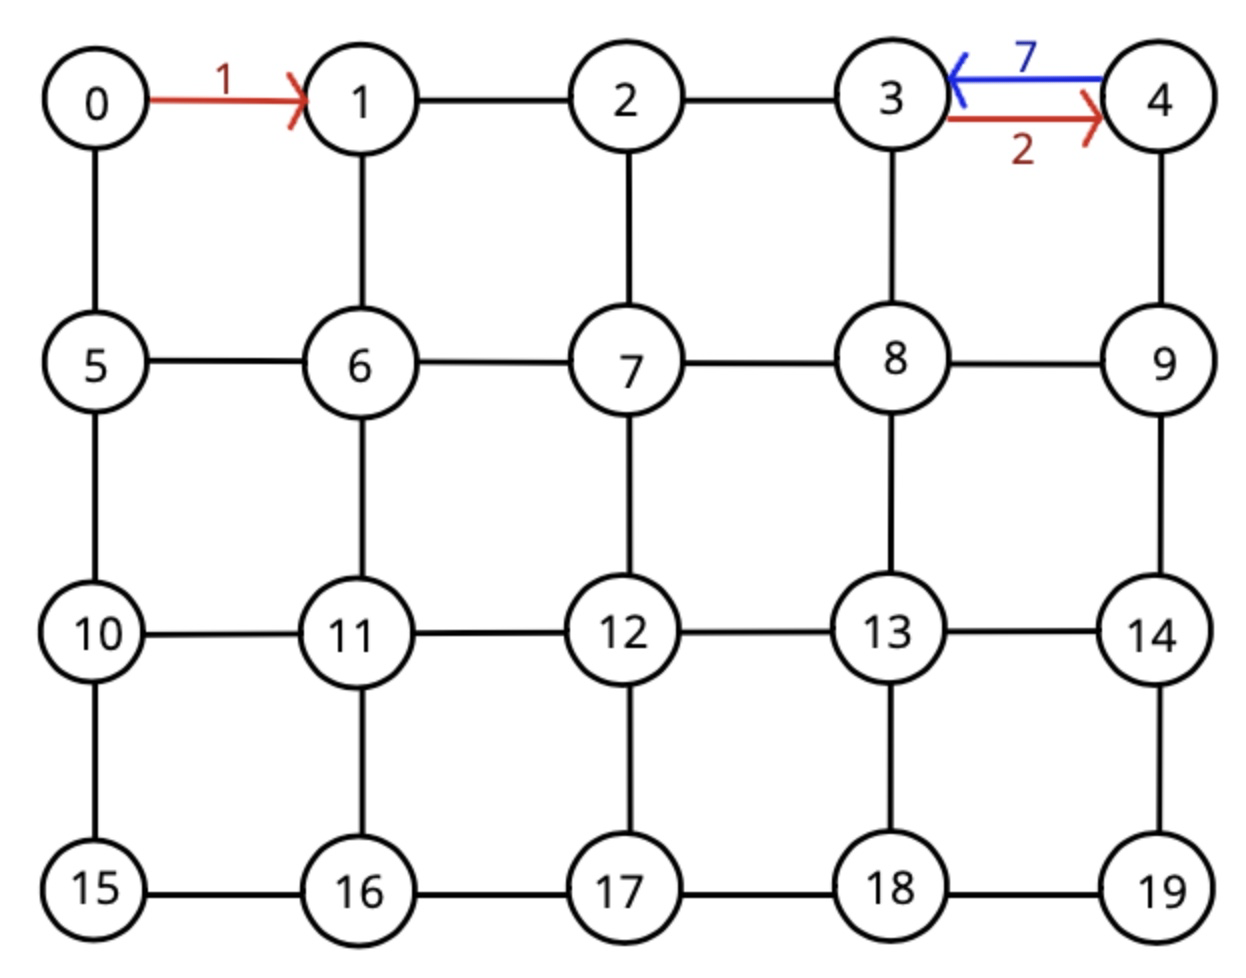
\includegraphics[scale=0.15]{graph.png}
            \caption{Przykład grafu typu "kartka w kratkę"}
        \end{center}
    \end{figure}
    W przeciwieństwie do jego odpowiednika napisanego w \texttt{C} program posiada interfejs graficzny użytkownika. Program będzie testowany za pomocą testów jednostkowych (JUnit oraz AssertJ).
    \newpage

    \section{Struktura głównego folderu}
    Struktura folderu jest stworzona zgodnie z wymaganiami programu \texttt{Maven}. Oprócz folderów typowych dla programów zarządzanych przez \texttt{Maven'a}
    znajduje się również folder zawierający dokumentację projektu.\newline
    \begin{forest}
        for tree={
          font=\ttfamily,
          grow'=0,
          child anchor=west,
          parent anchor=south,
          anchor=west,
          calign=first,
          inner xsep=7pt,
          edge path={
            \noexpand\path [draw, \forestoption{edge}]
            (!u.south west) +(7.5pt,0) |- (.child anchor) pic {folder} \forestoption{edge label};
          },
          before typesetting nodes={
            if n=1
              {insert before={[,phantom]}}
              {}
          },
          fit=band,
          before computing xy={l=15pt},
        }  
        [\texttt{Java}
          [\texttt{dokumentacja}
            [\texttt{Specyfikacja Implementacyjna}
                [\texttt{images}]
                [\texttt{listings}]
            ]
            [\texttt{Specyfikacja Funkcjonalna}
                [\texttt{images}]
                [\texttt{listings}]
            ]
            [\texttt{Sprawozdanie}
                [\texttt{images}]
                [\texttt{listing}]
            ]
          ]
          [\texttt{grapher}
            [\texttt{.idea}]
            [\texttt{src}
                [\texttt{main}
                  [\texttt{java}]
                  [\texttt{resources}]
                ]
            ]
            [\texttt{test}
              [\texttt{java}]
            ]
        ]
      ]
    \end{forest}

    \section{Funkcjonalności programu}
    \subsection{Pierwsze uruchomienie programu}
    Program podczas pierwszego uruchomienia ładuje główny ekran aplikacji. Ekran ten pozwala na generowanie oraz wczytywanie grafu z pliku, posiada on też pole pozwalające na wyświetlanie grafu.

    \subsection{Funkcjonalności programu}
    Program pozwala za pomocą intefejsu graficznego wybierać tryb generacji grafów, szukanie punktów na już wygenerowanym grafie oraz dokonywanie konfiguracji z menu ustawień.

    \subsection{Wyjście programu}
    W zależności od tego, czy użytkownik wybrał jeden z trybów generacji czy tryb do czytania wynik działania programu będzie inny.
    W trybach do generacji wyjściem będzie plik z wygenerowanym grafem oraz sam graf w oknie w interfejsie graficznym, natomiast w trybie do czytania będzie to wczytany graf z zaznaczoną najkrótszą ścieżką na nim w interfejscie graficznym oraz
    wypisana na ekranie ścieżka w formacie wybranym przez uzytkownika.
    \newpage

    \section{Interfejs graficzny użytkownika}
    Interfejst graficzny składa się z pięciu części. Poszczególne z nich to: 
    \begin{itemize}
      \item Wyświetlanie grafu -- w tym miejscu będzie wyświetlany graf,
      \item Generowanie grafu -- dostosowywanie ustawień generacji grafu,
      \item Plik -- wybór pliku z dysku,
      \item Szukanie najkrótszej ścieżki -- moduł odpowiedzialny za szukanie najkrótszej ścieżki między punktami,
      \item Informacja zwrotna dla użytkownika -- element wyświetlający informacje o niepoprawnych danych, generowaniu grafu itd.
    \end{itemize}
    \begin{figure}[ht]
      \begin{center}
          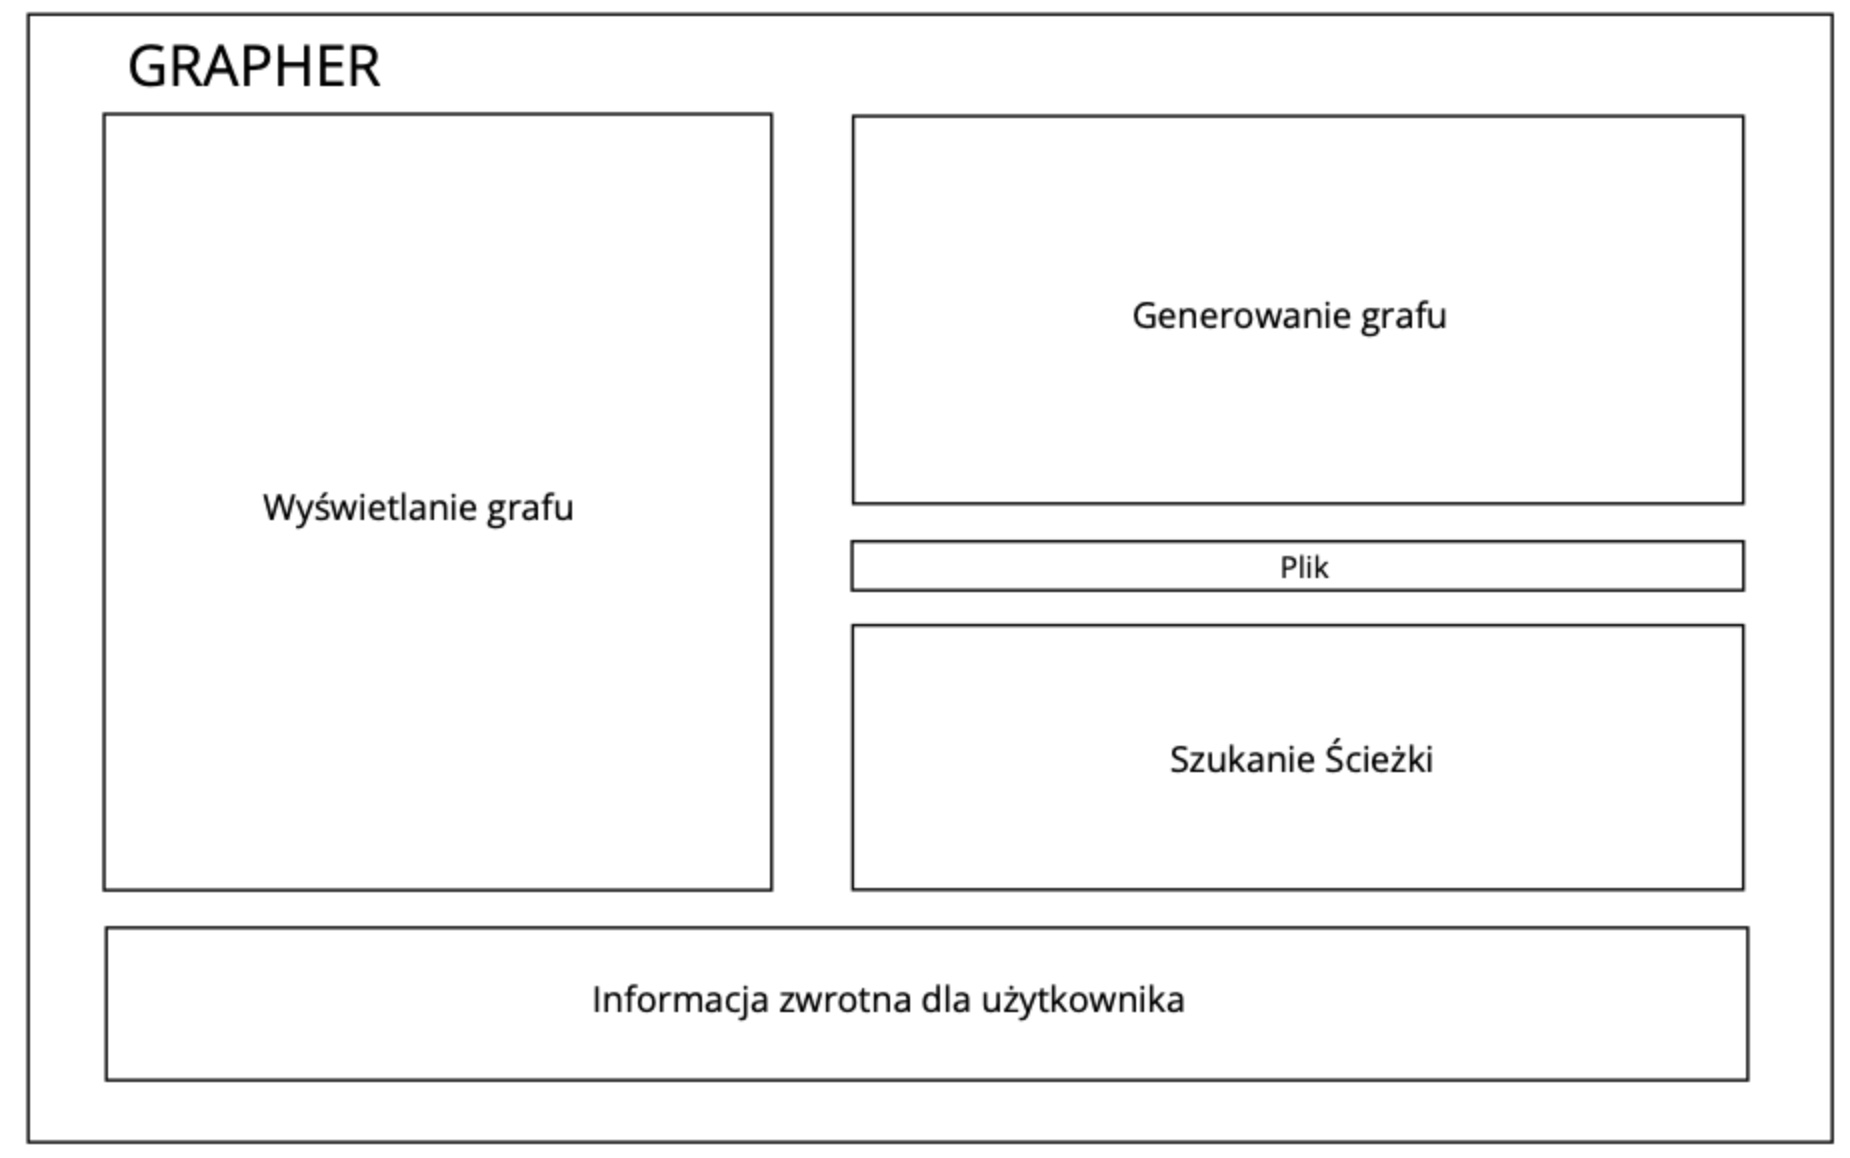
\includegraphics[scale=0.2]{gui_basic.jpg}
          \caption{Prosty rozkład GUI.}
      \end{center}
    \end{figure}
    \newpage

    \subsection{Generowanie grafu}
    Element ten odpowiedzialny jest za dostosowywanie ustawień generacji grafu, pozwala on na wybór ilości wierszy, kolumn, zakresu generacji wag krawędzi a także wybór trybu.
    \begin{figure}[ht]
      \begin{center}
          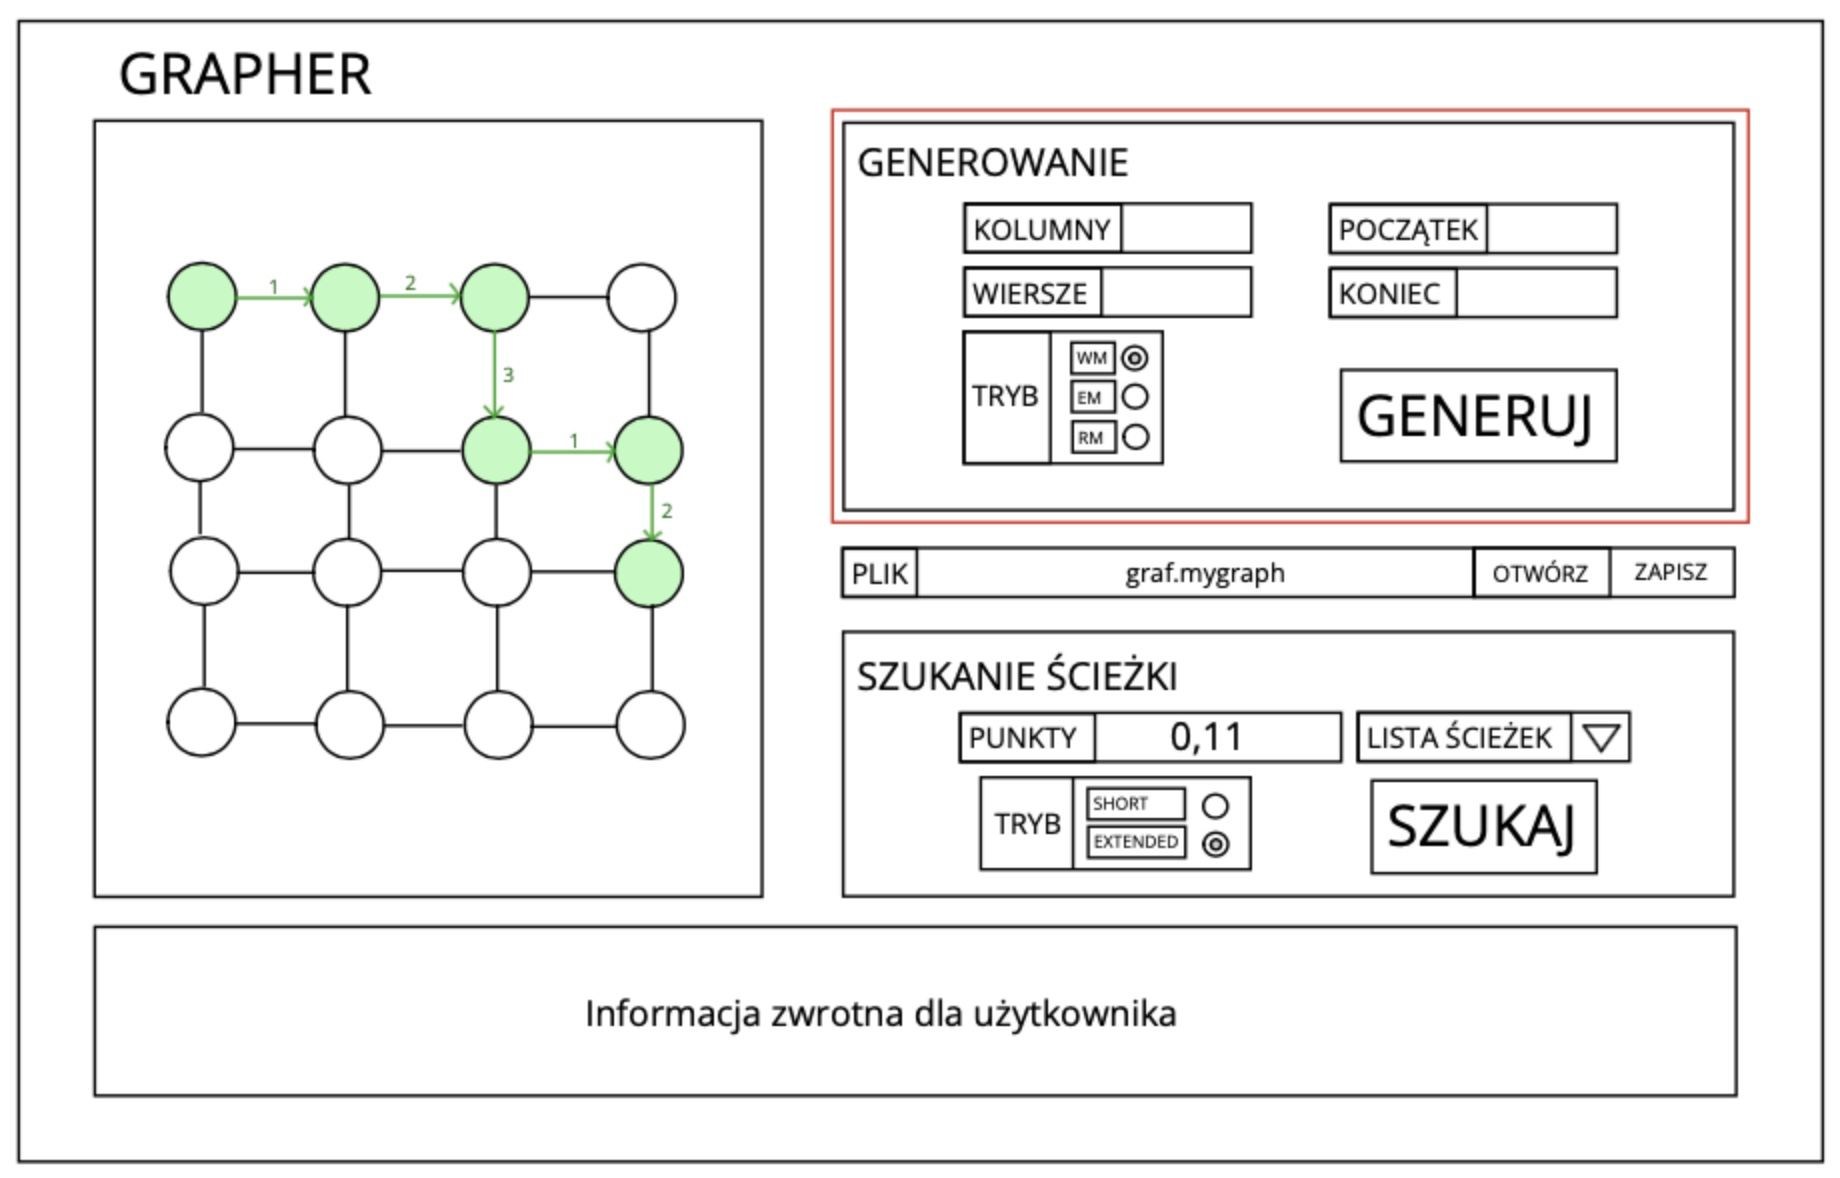
\includegraphics[scale=0.19]{gui_gen.jpg}
          \caption{Element odpowiedzialny za generowanie grafu.}
      \end{center}
    \end{figure}

    \subsection{Szukanie ścieżki}
    Element ten odpowada za szuaknie ścieżki między zadanymi punktami w aktualnei otwarym grafie. Element ten zawiera także rozwijane menu odpowiedzialne za kontrole jakie ścieżki wyświetlanie są aktualnie na grafie.
    \begin{figure}[ht]
      \begin{center}
          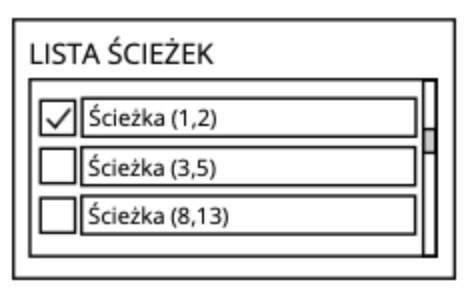
\includegraphics[scale=0.4]{gui_path_list.jpg}
          \caption{Lista ścieżek w aktualnie otwartym grafie.}
      \end{center}
    \end{figure}    
    \begin{figure}[ht]
      \begin{center}
          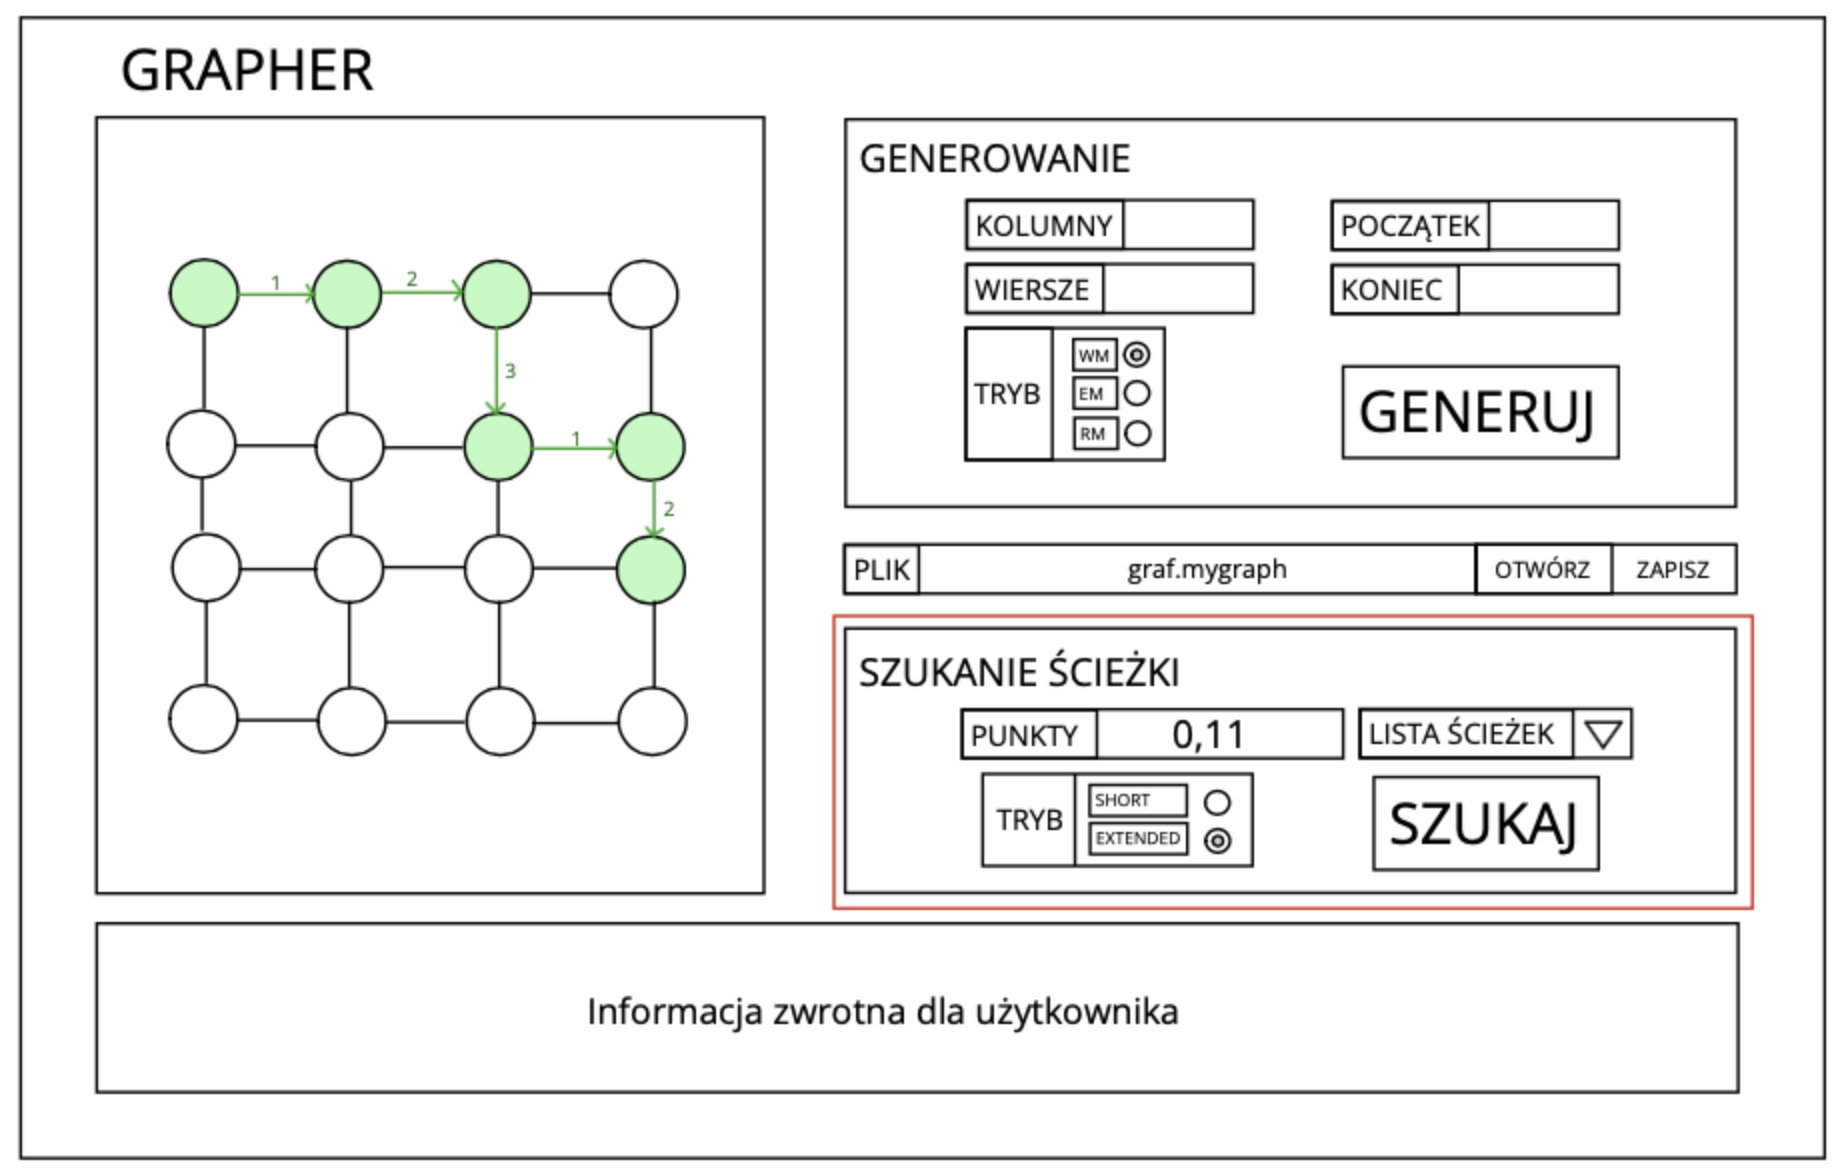
\includegraphics[scale=0.19]{gui_read.jpg}
          \caption{Element odpowiedzialny za szukanie najkrótszej ścieżki w grafie.}
      \end{center}
    \end{figure}
    \newpage
    
    \subsection{Wyświetlanie grafu}
    Po lewej stronie programu znajduje się obszar odpowiedzialny za wyświetlanie grafu, graf dopasowuje się rozmiarem do okienka.
    Gdy generowany graf jest za duży okno zamienia się w przesuwane aby umożliwić sprawne przeglądanie grafu.
    \begin{figure}[ht]
      \begin{center}
          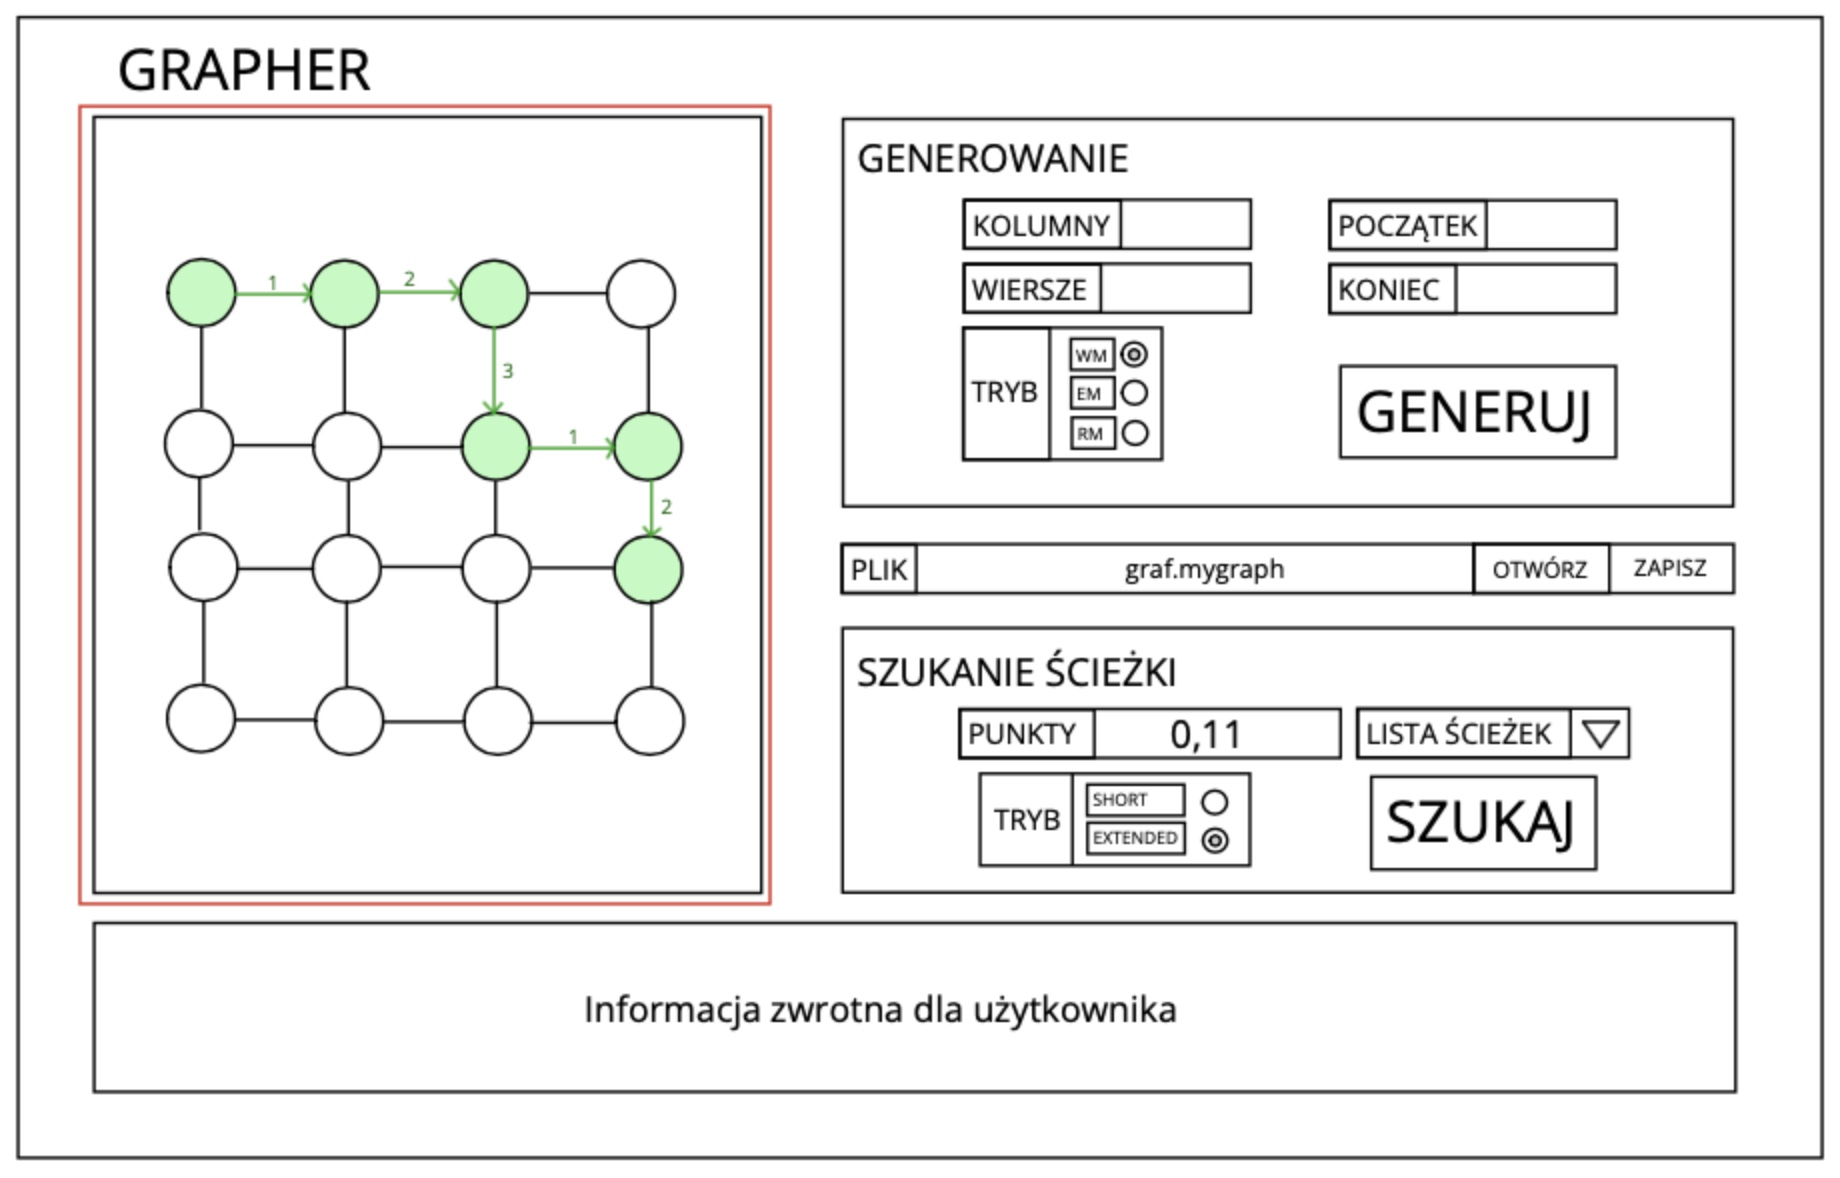
\includegraphics[scale=0.19]{gui_graph.jpg}
          \caption{Wyświetlany graf}
      \end{center}
    \end{figure}
    \newpage

    \section{Parametry programu}
    Niezależnie od dalszych potrzeb użytkownik musi wpierw określić z jakiego trybu będzie korzystał. Do wyboru mamy cztery tryby:
    \begin{itemize}
      \item WM -- Wage Mode,
      \item EM -- Edge Mode,
      \item ReM -- Random Mode,
      \item RM -- Read Mode.
    \end{itemize}
    Tryby można wpisać w całości z małych liter. Wszystkie tryby zostało dokładniej opisane w~ podrozdziale \textit{Cel projektu}.
    \newpage

    \subsection{Tryby generujące}
    \begin{enumerate}
      \item \texttt{[Plik]:}
      \newline Plik, do którego zostanie zapisany wygenerowany przez program graf, 
      plik będzie zawsze nadpisywany nową zawartością,
      
      \item \texttt{[Wiersze]:}
      \newline Liczba wierszy jakie zostaną wygenerowane w grafie. Liczba ta musi być większa od zera,
  
      \item \texttt{[Kolumny]:}
      \newline Liczba kolumn jakie zostaną wygenerowane w grafie. Liczba ta musi być większa od zera,
  
      \item \texttt{[Poczatek]:}
      \newline Początek przedziału z jakiego będą generowane wagi dla krawędzi między wierzchołkami. Musi to być wartość większa od 0,
  
      \item \texttt{[Koniec]:}
      \newline Koniec przedziału z jakiego będą generowane wagi dla krawędzi między wierzchołkami. Musi to być wartość większa od 0.
    \end{enumerate}

    \subsection{Tryb do czytania}
    \begin{enumerate}
      \item \texttt{[Plik]:}
      \newline Plik, z którego jest wczytywany graf oraz szukana jest w nim najkrótsza ścieżka,

      \item \texttt{[Tryb wyświetlania]:}
      \newline Wymagany tryb wyświetlania ścieżki wybieramy spośród poniższych:
      \begin{itemize}
          \item \texttt{standard} – tryb pozwala na wyświetlenie skróconej wersji najkrótszej ścieżki między dwoma zadanymi punktami.
          \newline Format wyświetlania: (od,do); od $\rightarrow$ następny punkt $\rightarrow$ ... $\rightarrow$ do
          \newline \textbf{np.}
          \newline(7,8); 7 $\rightarrow$ 6 $\rightarrow$ 5 $\rightarrow$ 9 $\rightarrow$ 8,
          \item \texttt{extended} -- tryb pozwala na wyświetlenie rozszerzonej wersji najkrótszej ścieżki między dwoma zadanymi punktami.
          \newline Format wyświetlania: (od,do); (od,do); od(waga przejścia) $\rightarrow$ następny punkt(waga przejścia) $\rightarrow$ ... $\rightarrow$ do
          \newline \textbf{np.}
          \newline (7,8); 7(0,4) $\rightarrow$ 6(0,2) $\rightarrow$ 5(0,3) $\rightarrow$ 9(0,1) $\rightarrow$ 8.
    \end{itemize}
      \item \texttt{[Najkrótsza ścieżka]:}
      \newline Trzeba podać pary punktów między, którymi szukamy najkrótszej ścieżki w grafie.
    \end{enumerate}

    \subsection{Format pliku do czytania}
    Program do działania w trybie Read Mode przyjmuje plik o określonych właściwościach:
    \begin{itemize}
        \item W pierwszym wierszu pliku znajduje się informacja o liczbie wierszy i kolumn jakie składają się na graf,
        \item W każdym następnym wierszu znajduję się informacja o tym z jakimi innymi wierzchołkami połączony jest dany wierzchołek oraz waga jaka odpowiada temu połączeniu.
    \end{itemize}
    Ze względu na numerowanie wierzchołków od zera, numer wiersza odpowiada numerowi wierzchołka zwiększonego o jeden. 
    \newpage
    Przykładowa zawartość pliku:
    \lstinputlisting{listings/format.txt}

    \section{Przykładowe scenariusze działania programu}
    \subsection{Dla trybu generującego}
    Użytkownik wybiera tryb do generowania spośród trzech rożnych. Następnie wpisuje w okno liczbę wierszy oraz kolumn, podaje plik oraz poczatek i koniec przedziału z jakiego losowane są wagi
    krawędzi. Program wyświetla wygenerowany graf w oknie i zapisuje go do pliku podanego przez użytkownika.
  
    \begin{figure}[ht]
      \begin{center}
          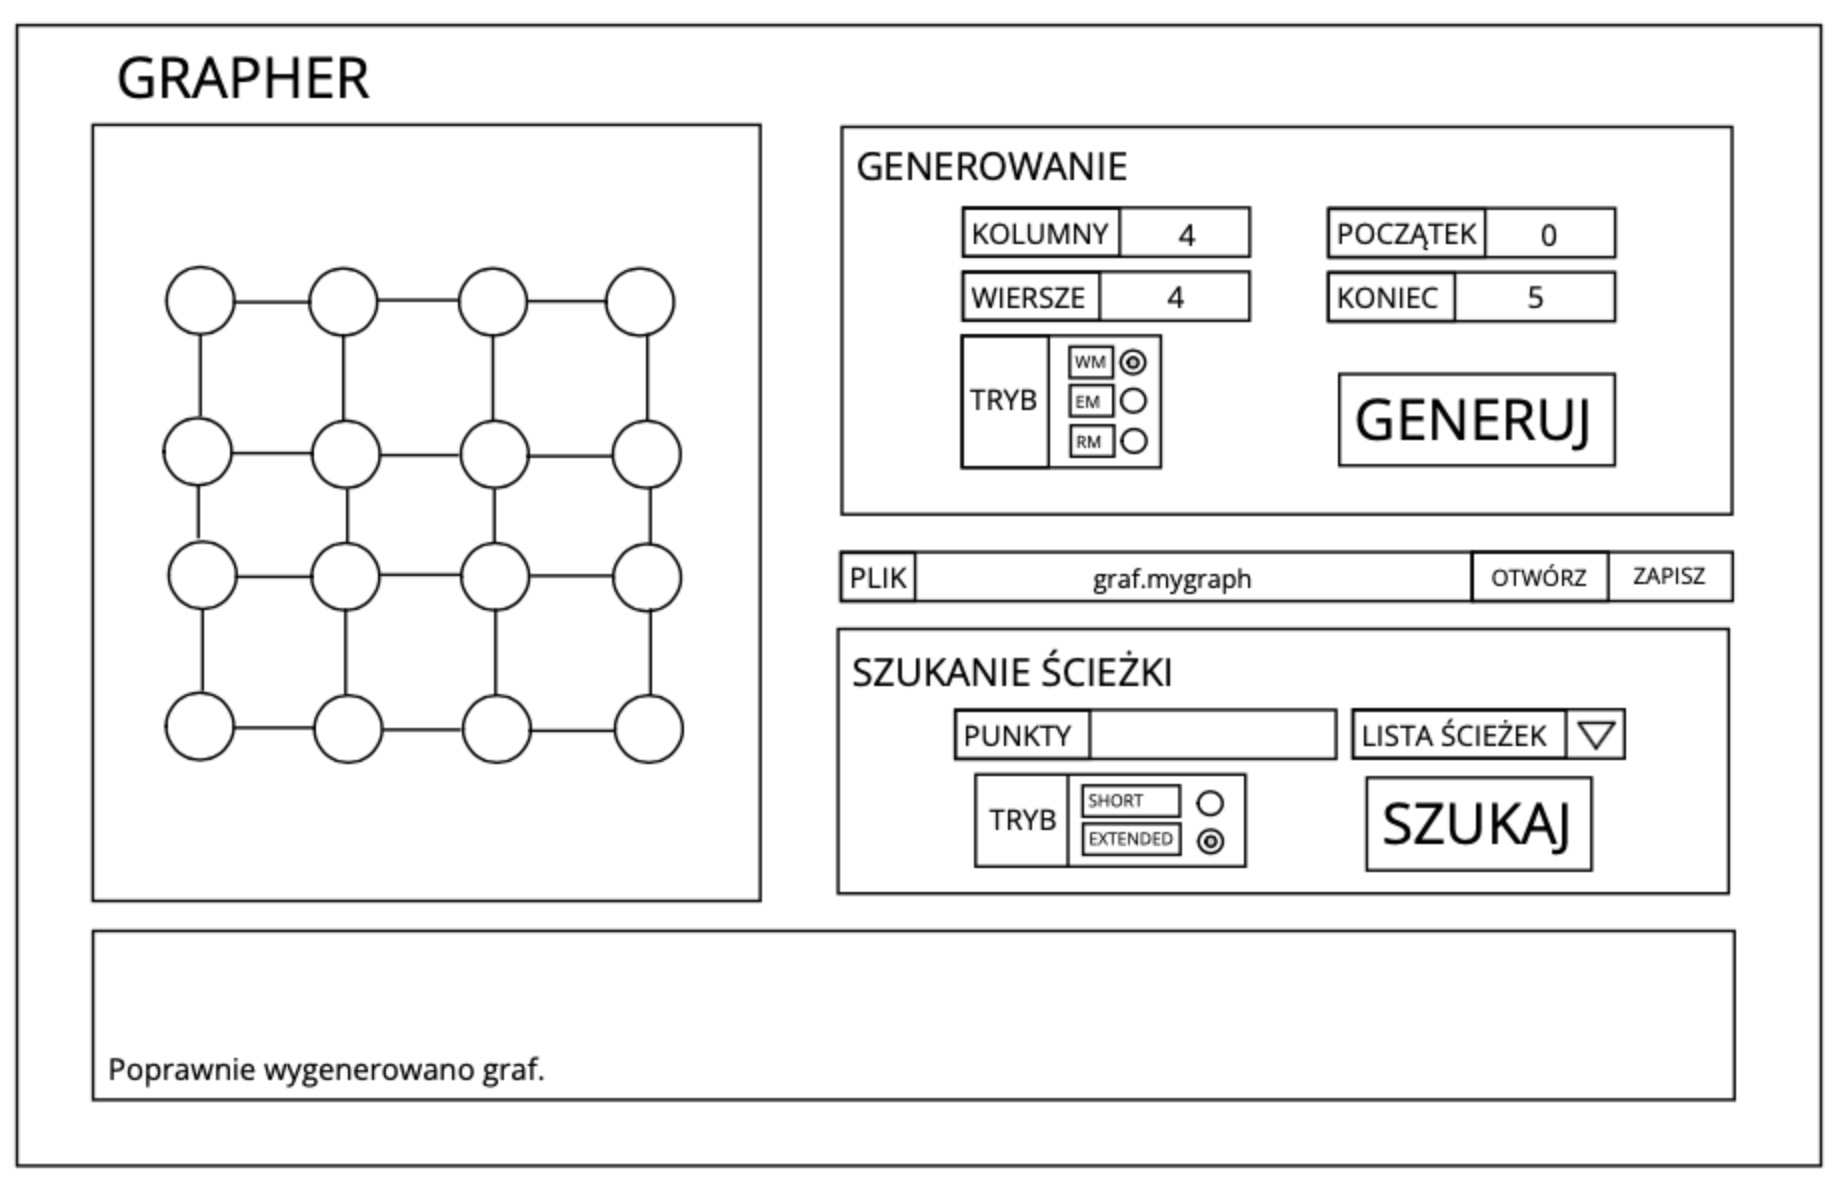
\includegraphics[scale=0.22]{example_gen.jpg}
          \caption{Przykładowe generowanie grafu.}
      \end{center}
    \end{figure}
    \newpage

    \subsection{Dla trybu do czytania}
    Użytkownik wybiera tryb do czytania, a następnie wprowadza plik z grafem i punkty między, którymi będzie szukana najkrótsza ścieżka. Nie można zapomnieć o podaniu trybu w jaki będzie wyświetlana najkrótsza scieżka w formie tekstowej.
    Program wyświetli graf w oknie i zaznaczy najkrótszą ścieżkę między punktami oraz wypisze ją w odpowiednim oknie zgodnie z podaną przez użytkownika trybem.
    \begin{figure}[ht]
      \begin{center}
          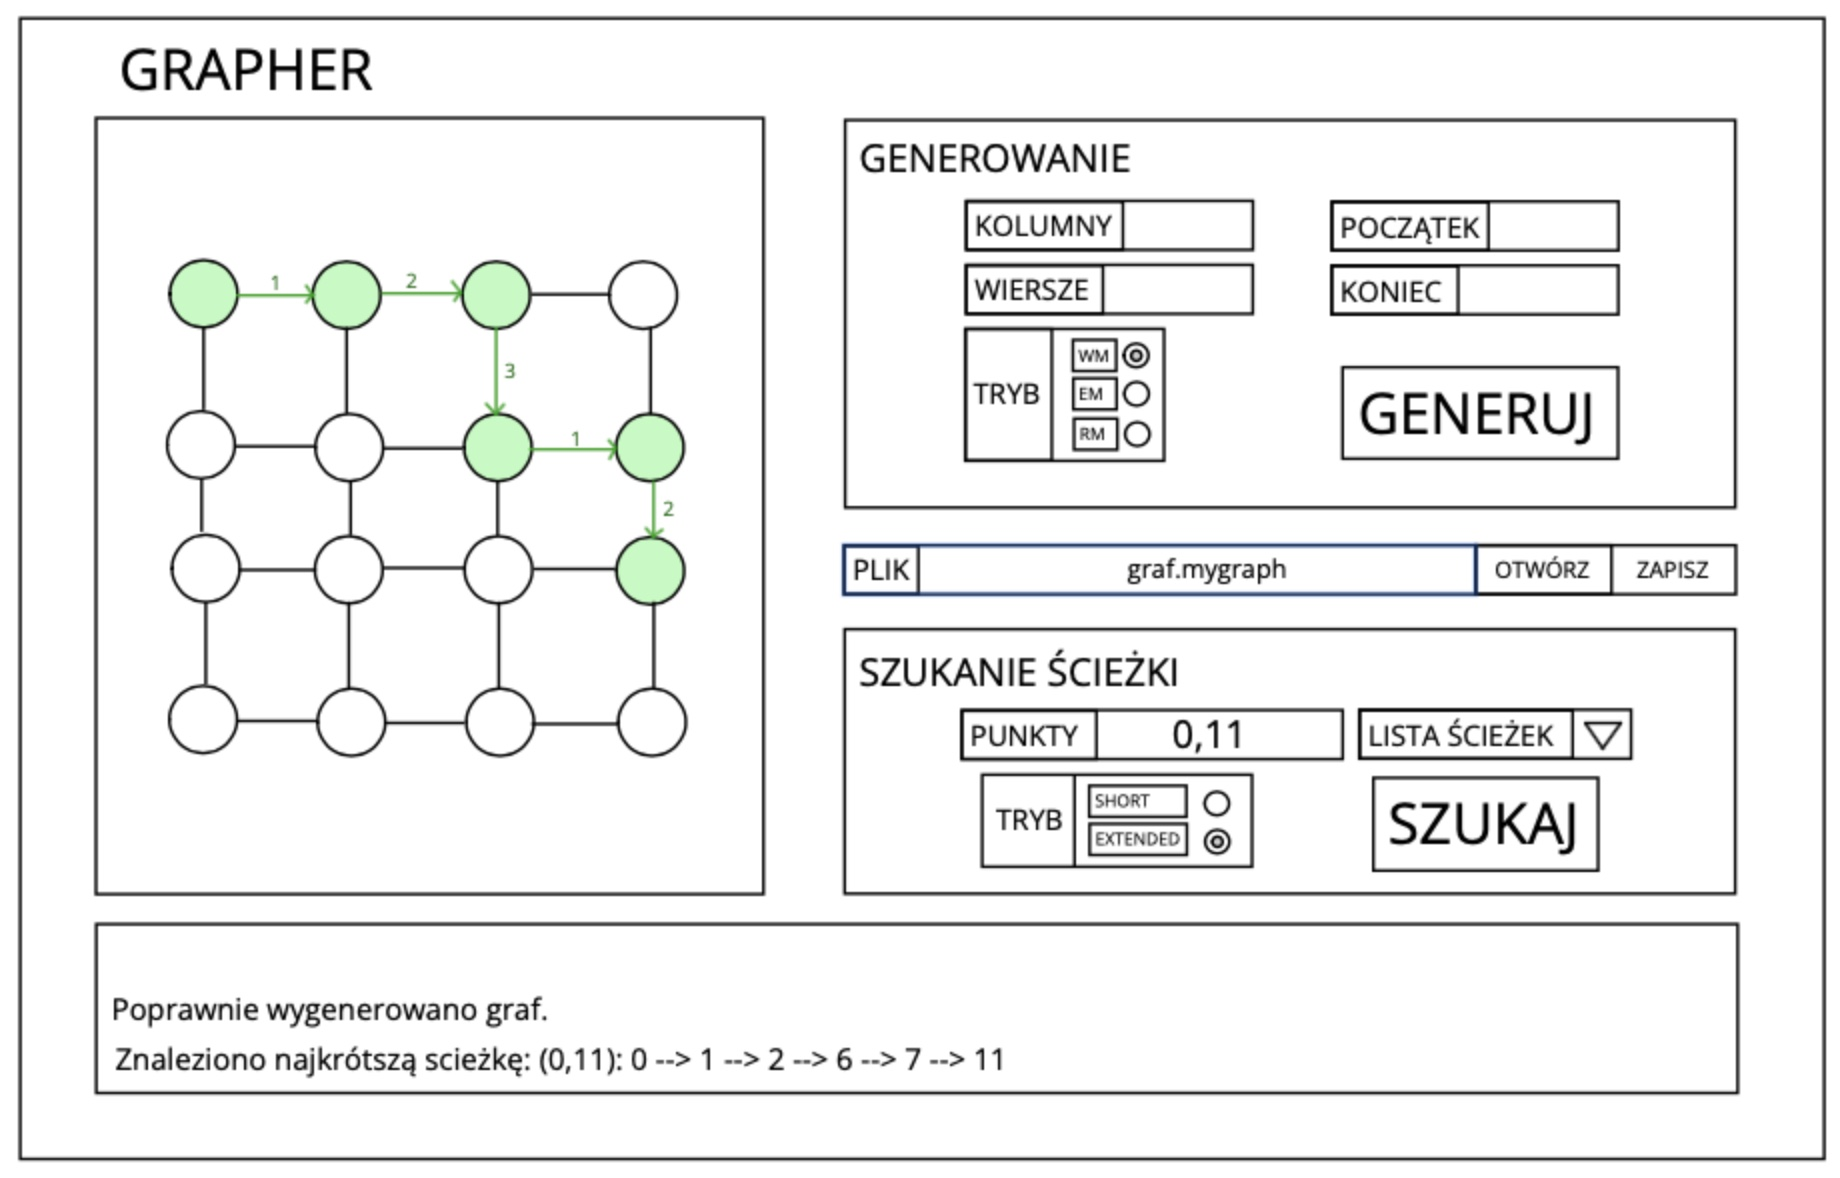
\includegraphics[scale=0.22]{example_pathfinding.jpg}
          \caption{Przykładowe szukanie ścieżki w grafie.}
      \end{center}
    \end{figure}
    \newpage

    \section{Obsługiwane błędy}
    Błędy obslugiwane przez program w Javie są takie same jak jego odpowiednik w C. Listę błędów zamieszczamy poniżej.
    \newline \begin{tabularx}{\textwidth}{ l|c|X } 
        \hline Nazwa Błędu & Kod & Wyjaśnienie błędu\\ 
        \hline NO\_MODE\_FOUND & 226 & Niepoprawny tryb lub jego brak\\
        \hline NO\_FILE\_FOUND & 231 & Nie podano pliku\\ 
        \hline WRONG\_NUM\_OF\_ROWS & 232 & Podano niepoprawną liczbę wierszy\\
        \hline WRONG\_NUM\_OF\_COL & 233 & Podano niepoprawną liczbę kolumn\\
        \hline WRONG\_RANGE\_OF\_WAGES & 234 & Zły zakres losowania wartości wag\\
        \hline NO\_FLAG\_FOUND & 235 & Nie podano trybu wyświetlania ścieżki w trybie Read Mode\\
        \hline WRONG\_POINTS & 228 & Podano nieistniejący punkt lub ich złą liczbę\\
        \hline NO\_COHERENT & 237 & Graf jest niespójny \\
        \hline NULL\_POINTER\_EXCEPTION & 228 & Alokacja pamięci się nie udała\\
        \hline INVALID\_DATA & 225 & Nie podano wymaganych argumentów\\
        \hline NO\_COL\_ROWS\_FOUND & 223 & W pliku do czytania nie znaleziono kolumn lub wierszy\\
        \hline NO\_NODES\_FOUND & 220 & W trybie nie znaleziono wierzchołków\\
        \hline WRONG\_ROWS\_COLUMNS & 198 & W czytanym pliku kolumny lub wiersze mają wartość mniejszą równą 0\\
        \hline
    \end{tabularx}

\end{document}